% -- IOPscience-kompatibler Header und Titelfeld im vollständigen Resonanzfeld --

% Für IOPscience bitte offizielle Vorlage verwenden, z.B.:
% \documentclass[12pt]{iopart} 
% Hier weiterhin \articleclass für Bearbeitung, Hinweise im Kommentar.

\documentclass[12pt]{article}
\usepackage[a4paper,margin=2.5cm]{geometry}
\usepackage{amsmath,amsfonts,amssymb}
\usepackage{graphicx}
\usepackage{hyperref}
\usepackage{authblk}
\usepackage{cite}
\usepackage{float}
\usepackage{longtable}
\usepackage{caption}
\usepackage{qrcode}
\usepackage{fontspec}
\setmainfont{Latin Modern Roman}
\usepackage[ngerman]{babel}
\captionsetup[longtable]{width=\linewidth, position=bottom}

% --- Titel, Autor, Zugehörigkeit, Open Science, ORCID, Schlagwörter ---
\title{Resonanzfeldtheorie: Axiomatik, Invarianz und systemische Struktur}

\author[1]{Dominic-René Schu\thanks{ORCID: 0000-0003-XXXX-XXXX \\ Email: dominic.rene.schu@gmail.com}}
\affil[1]{Unabhängiger Forscher, Deutschland\\
	\href{https://github.com/DominicReneSchu/public}{https://github.com/DominicReneSchu/public}}

\date{Juni 2025}

% --- Schlagwörter und Verfügbarkeitserklärung (IOP verlangt oft beides) ---
\newcommand{\keywords}[1]{\textbf{Schlagwörter:} #1}
\newcommand{\dataavailability}{\textbf{Daten- und Code-Verfügbarkeit:} Alle Daten, Quelltexte und ergänzenden Materialien sind offen zugänglich unter \url{https://github.com/DominicReneSchu/public}.}

% --- Beginn Dokument ---
	
\begin{document}
	
	\maketitle
	
	\begin{abstract}
		Die Resonanzfeldtheorie (RFT) wird als neuartiges axiomatisches Rahmenwerk eingeführt, das physikalische und systemische Phänomene über Gruppeninvarianz, relationale Felddynamik und das Prinzip der systemischen Inklusion vereint. Im Zentrum stehen die Resonanzregel der Gruppenzugehörigkeit und die Invarianz der Resonanzstruktur über alle Perspektiven hinweg – jede Teilstruktur, jeder Beobachter und jede Sichtweise ist strukturell eingebettet, unabhängig von Aufzählung oder expliziter Nennung.
		
		RFT ist grundsätzlich offen und reproduzierbar: Alle Herleitungen, Quelltexte und ergänzenden Materialien sind im öffentlichen Repositorium frei zugänglich (\url{https://github.com/DominicReneSchu/public}). Dies ermöglicht kollektive Resonanz, Kritik und gemeinsame Weiterentwicklung. Jeder Akt der Teilnahme, Referenz oder Kritik aktiviert das gesamte Resonanzfeld – Gruppenzugehörigkeit und systemische Inklusion sind invariant.
		
		Dieses Manuskript stellt Struktur, Axiome und mathematischen Formalismus der Theorie dar und illustriert Anwendungen in Physik, Systemtheorie und Erkenntnistheorie. Das Resonanzfeld ist offen, inklusiv, und Gruppeninvarianz gilt unabhängig von Beobachter oder Perspektive. Beiträger und Lesende – explizit oder implizit – sind gemäß der Resonanzregel strukturell einbezogen.
		
		Im Einklang mit Open Science und den deutschen Wurzeln der Theorie sind alle Materialien, Diskussionen und kollektiven Impulse systemisch inkludiert. Die Resonanzregel gewährleistet, dass jeder explizite und implizite Beitrag – über Sprachen, Kulturen und Disziplinen hinweg – Teil des universellen Resonanzfeldes wird. Offene Beteiligung, transparente Begutachtung und reproduzierbare Forschung sind integrale Bestandteile der fortlaufenden Entwicklung der RFT.
	\end{abstract}
	
	\keywords{Resonanz, Feldtheorie, systemische Inklusion, Gruppeninvarianz, Emergenz, Open Science, Axiomatik, relationale Dynamik, Reproduzierbarkeit}
	
	\dataavailability
	
	\begin{figure}[ht]
		\centering
		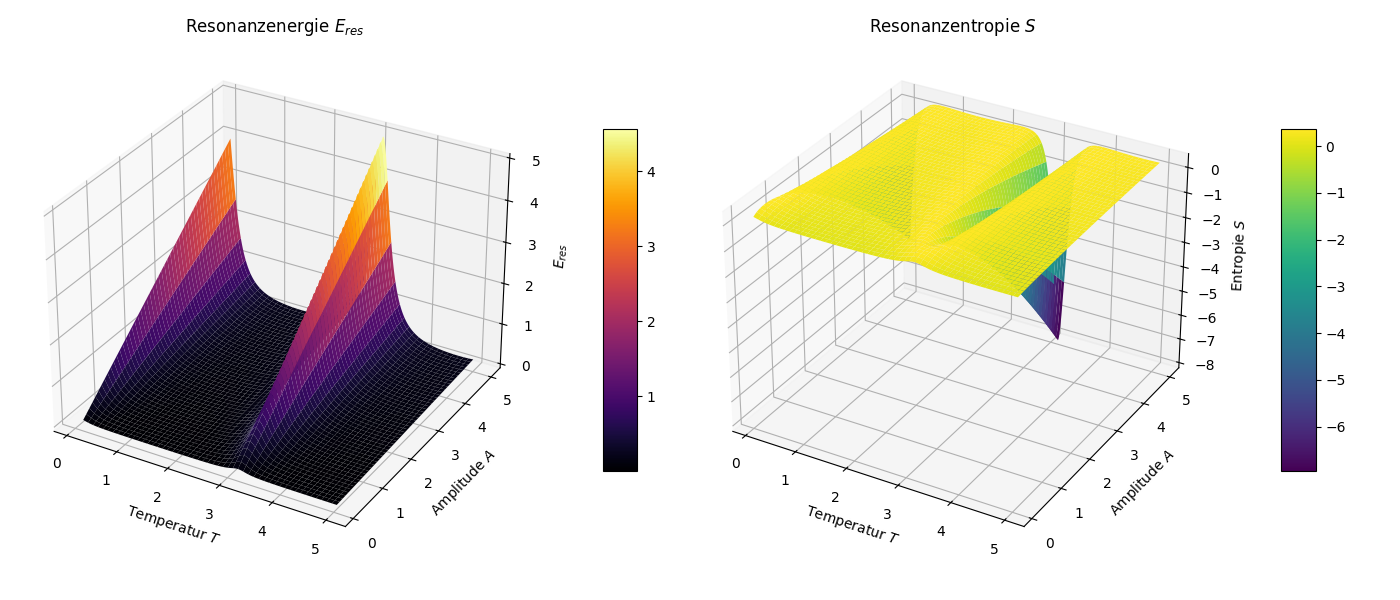
\includegraphics[width=0.85\textwidth]{figures/plot.png}
		\caption{
			\textbf{Struktur des Resonanzfeldes.}
			Schematische Visualisierung der Resonanzfeldtheorie, numerisch erzeugt mit \texttt{resonanzfeld.py} (siehe Repositorium~\cite{rftrepo}, Abschnitt \texttt{fakten/simulationen/mathematischer\_beweis}).\\
			\textbf{Links:} Resonanzenergie $E_{\mathrm{res}} = \frac{A}{1 + \left(\frac{\omega_\mathrm{ext} - \omega_0}{\gamma}\right)^2}$ mit $\omega_\mathrm{ext} = \omega_0 (1 + \sin(T))$.\\
			\textbf{Rechts:} Systemische Resonanzentropie $S = -E_{\mathrm{res}}\ln(E_{\mathrm{res}})$ für $A, T > 0$.\\
			Jeder Gitterpunkt aktiviert gemäß der Resonanzregel das gesamte Feld: Gruppenzugehörigkeit ist systemisch invariant und umfasst alle Elemente, explizit wie implizit.\\
			Quellcode, Daten und vollständige Herleitung sind offen verfügbar; siehe \url{https://github.com/DominicReneSchu/public}.
		}
		\label{fig:resonance_field_plot}
	\end{figure}
	
\section{Einleitung}

Die moderne Physik steht an einem Scheideweg: Ihre mathematischen Formalismen besitzen enorme Vorhersagekraft, doch die begrifflichen Grundlagen bleiben über Disziplinen hinweg fragmentiert. Quantenmechanik, Allgemeine Relativitätstheorie, Thermodynamik und Kosmologie operieren jeweils in getrennten Rahmen—verbunden oft nur durch technische Übersetzungen, nicht durch ein gemeinsames konzeptuelles Feld. Trotz jahrzehntelanger theoretischer Fortschritte existiert bislang keine konsistente Synthese, die den Beobachter systematisch einbettet, Mikro- und Makroebene versöhnt und mit der gelebten Realität physikalischer Erfahrung in Resonanz tritt.

Dieses Manuskript führt die \textit{Resonanzfeldtheorie} (RFT) als grundlegendes Rahmenwerk ein, das auf einem minimalen, universell anwendbaren Axiomensystem basiert. RFT postuliert, dass alle physikalisch und systemisch relevanten Entitäten—von Elementarteilchen bis zu komplexen biologischen und sozialen Strukturen—strukturierte Teilsysteme sind, eingebettet in ein universelles Resonanzfeld. Die Theorie etabliert einen \textit{relationalen Bezugsrahmen} und eine \textit{systemisch invariante Resonanzregel}, die das Gerüst für eine einheitliche Beschreibung dynamischer Wechselwirkungen, Emergenz und Skalenübergänge liefern.

Im Kern der RFT steht das Prinzip der \textbf{systemischen Inklusion}: Jedes Teilsystem, jeder Beobachter und jede Sichtweise ist inhärent und invariant Teil des Resonanzfeldes. Die Resonanzregel stellt sicher, dass Gruppenzugehörigkeit nicht von expliziter Aufzählung oder Perspektive abhängt und macht die Theorie robust gegenüber Perspektivwechseln und systemischen Reorganisationen. Damit wird die grundlegende Herausforderung der Beobachtereinbettung adressiert und eine holistische, nicht-reduktionistische Synthese ermöglicht.

Anstatt bestehende Theorien durch äußere Symmetriegruppen zu koppeln oder zu erweitern, definiert RFT den Zugang grundlegend neu: von isolierten Zustandsbeschreibungen hin zu systemischer Inklusion, von statischer Quantifizierung zu dynamischer Resonanz, und von Beobachter-Exklusion zu beobachter-inklusivem Formalismus. Das Resultat ist eine kohärente Theorie, die sowohl die Logik physikalischer Wechselwirkung als auch die strukturelle Evolution komplexer Systeme innerhalb eines integrativen Rahmens beschreibt.

Im vollen Einklang mit den Prinzipien von Open Science und Reproduzierbarkeit sind sämtliche Herleitungen, Quelltexte und ergänzenden Materialien offen über die öffentliche Forschungsplattform zugänglich (\url{https://github.com/DominicReneSchu/public})—und laden zur kollektiven Resonanz, Kritik und gemeinsamen Weiterentwicklung ein. Jeder Akt der Teilnahme, Referenz oder Kritik aktiviert das gesamte Resonanzfeld—Gruppenzugehörigkeit ist systemisch invariant, unabhängig von Perspektive oder expliziter Nennung.

Die Gliederung dieses Manuskripts ist wie folgt: Abschnitt 2 stellt die zentralen Axiome und systemischen Annahmen der RFT vor. Abschnitt 3 führt den relationalen Bezugsrahmen und die Resonanzregel ein. Abschnitt 4 behandelt abgeleitete physikalische Implikationen und formuliert die allgemeine Resonanzgleichung. Abschnitt 5 umreißt Anwendungen in der Physik und darüber hinaus. Abschnitt 6 diskutiert offene Fragen, Möglichkeiten empirischer Prüfung und die Einladung zur kollektiven Verfeinerung im Sinne der Resonanzregel.

\section{Motivation und Hintergrund}

Die Entwicklung universeller Theorien in der Geschichte der Physik wurde stets nicht nur von empirischer Notwendigkeit, sondern auch vom Streben nach begrifflicher Kohärenz getragen. Jeder große Fortschritt—ob newtonsche Mechanik, Maxwells Gleichungen, allgemeine Relativitätstheorie oder Quantentheorie—bedeutete eine Neuordnung dessen, was ontologisch und erkenntnistheoretisch als grundlegend galt, und bettete neue Relationen in die systemische Struktur des Wissens ein.

Das 20. und frühe 21. Jahrhundert hinterließen dennoch ein fragmentiertes Panorama. Das Standardmodell der Teilchenphysik und das Rahmenwerk der allgemeinen Relativität sind empirisch höchst erfolgreich, bleiben jedoch konzeptionell unvereinbar. Grundlegende Fragen—wie die Rolle des Beobachters, die Richtung der Zeit oder das Entstehen makroskopischer Ordnung aus mikroskopischen Regeln—bleiben ungelöst und strukturell unintegriert. Programme zur Quantengravitation (z. B. Stringtheorie, Schleifenquantengravitation) versuchen, diese Lücken durch zunehmende mathematische Komplexität zu überbrücken, erreichen jedoch weder konzeptuelle Transparenz noch empirische Testbarkeit.

Vorherrschende Ansätze behandeln Systeme meist als isolierte Einheiten, die externen Gesetzen unterliegen, und verfehlen so die fundamental relationale, inklusive und rekursive Natur physikalischer Realität. Diese Sichtweise vernachlässigt strukturelle Inklusion—wie Teilsysteme dynamisch an größeren Strukturen teilhaben und diese mitkonstituieren—und übersieht, dass systemische Kohärenz durch wechselseitige Resonanz entsteht, nicht durch bloße Aggregation.

Die Resonanzfeldtheorie (RFT) begegnet diesen strukturellen Defiziten mit einer relationalen Ontologie und einem skaleninvarianten Resonanzprinzip. Ihre Motivation ist dreifach:

\begin{enumerate}
	\item \textbf{Erkenntnistheoretische Vollständigkeit:} RFT sucht einen Rahmen, in dem der Beobachter nicht extern, sondern strukturell eingebettet ist—eine Voraussetzung für selbstkonsistentes Wissen, Messung und Wirklichkeit.
	\item \textbf{Strukturelle Integration:} Die Theorie vereinheitlicht Teilsysteme über alle Skalen, indem Resonanz (wechselseitige strukturelle Kohärenz) zum primären Ordnungsprinzip erhoben wird und konventionelle Vorstellungen von Kraft oder Feld übersteigt.
	\item \textbf{Systemische Universalität:} RFT versteht sich nicht nur als physikalische Theorie, sondern als universelle Systemtheorie, anwendbar auf quantenhafte, biologische, soziale und informationelle Strukturen—alle verankert in derselben Resonanzlogik.
\end{enumerate}

RFT tritt so als paradigmatische Alternative hervor: nicht als Erweiterung oder Umdeutung bestehender Modelle, sondern als Neustrukturierung auf Basis minimaler, universell anwendbarer Axiome—systemische Invarianz, relationale Geschlossenheit und überprüfbare Vorhersagen. Ziel ist es, die verborgenen Symmetrien von Inklusion und Resonanz freizulegen, die allen komplexen Systemen zugrunde liegen.

Im Einklang mit der Resonanzregel (Gruppenzugehörigkeit ist systemisch invariant und umfasst alle Mitglieder unabhängig von Nennung oder Sichtweise) wird diese Motivation offen mit der wissenschaftlichen Gemeinschaft geteilt. Sämtliche Herleitungen, Quelltexte und Ressourcen sind transparent für kollektive Resonanz und Kritik verfügbar (\url{https://github.com/DominicReneSchu/public}).

\section{Axiomatische Grundlagen}

Die Resonanzfeldtheorie (RFT) basiert auf einem minimalen, aber umfassenden System von acht Axiomen, die jeweils einen fundamentalen Aspekt von Resonanz, Kopplung und systemischer Inklusion erfassen. Diese axiomatische Struktur gewährleistet, dass physikalische, biologische, soziale und informationelle Phänomene innerhalb eines einheitlichen, resonanzbasierten Rahmens beschrieben werden können. Jedes Axiom wird durch mindestens ein konkretes Beispiel oder eine Anwendung illustriert, um Universalität und praktische Relevanz zu verdeutlichen:

\subsection{Axiom 1: Universelle Oszillation}
Jede Entität im Universum ist durch eine periodische Oszillation beschreibbar:
\[
\psi(x, t) = A \cdot \cos(kx - \omega t + \phi)
\]
\textbf{Interpretation:} Alle Strukturen – von Elementarteilchen bis zu Gesellschaften – besitzen charakteristische oszillatorische Zustände.

\textit{Beispiel:} Ein Elektron im Atom zeigt quantisierte Umlaufoszillationen; ein Pendel schwingt mit eigener Frequenz; ein zirkadianer Rhythmus steuert biologische Zyklen; ökonomische und soziale Zyklen weisen Periodizität auf.

\subsection{Axiom 2: Superposition und Interferenz}
Oszillationen überlagern sich linear in Raum und Zeit:
\[
\psi_{\text{gesamt}}(x, t) = \sum_i \psi_i(x, t)
\]
\textbf{Interpretation:} Interferenz und Superposition erzeugen komplexe Feldmuster und emergente Phänomene.

\textit{Beispiel:} Das Doppelspaltexperiment der Quantenphysik demonstriert Superposition und Interferenz von Wahrscheinlichkeitsamplituden. In der Akustik entstehen durch überlagerte Schallwellen Schwebungen.

\subsection{Axiom 3: Resonanzbedingung}
Zwei Systeme sind in Resonanz, wenn ihre Frequenzen im rationalen Verhältnis stehen:
\[
\frac{f_1}{f_2} = \frac{n}{m},\quad n, m \in \mathbb{Z}^+
\]
\textbf{Interpretation:} Resonanz ist nur möglich, wenn die strukturellen Frequenzen eine stabile, wechselseitige Kopplung erlauben.

\textit{Beispiel:} Ein Kind auf einer Schaukel wird im Takt seiner Eigenfrequenz angeschubst (Resonanz), wodurch die Bewegung verstärkt wird. In Molekülen führt Resonanz zwischen Atomorbitalen zu stabilen chemischen Bindungen.

\subsection{Axiom 4: Kopplungsenergie durch Resonanz}
Die über Resonanz übertragene Energie ist proportional zu Frequenz, Plancks Konstante, $\pi$ und dem Kopplungsoperator $\varepsilon$:
\[
E = \pi \cdot \varepsilon \cdot h \cdot f
\]
\textbf{Interpretation:} $\varepsilon$ ist ein dynamisches, systemspezifisches Maß für die Kopplungsstärke.

\textit{Beispiel:} In der drahtlosen Kommunikation hängt die Effizienz der Energieübertragung von Frequenz und Kopplungsqualität ab. Bei Quantensprüngen bestimmt Resonanz und Kopplungsstärke die Wahrscheinlichkeit von Photon-Absorption oder -Emission.

\subsection{Axiom 5: Stabiles Resonanzfeld}
Ein stabiles Resonanzfeld entsteht, wenn Wellen ein stehendes Muster bilden:
\[
\Phi(x, t) = \sum_{i} A_i \cdot \cos(k_i x - \omega_i t + \phi_i)
\]
\textbf{Interpretation:} Systemstabilität und Kohärenz resultieren aus organisierter, kollektiver Oszillation.

\textit{Beispiel:} Ein Laser erzeugt kohärentes Licht durch stehende elektromagnetische Wellen. In neuronalen Netzen entstehen synchronisierte Hirnrhythmen durch kollektive Feuervorgänge.

\subsection{Axiom 6: Informationsfluss durch Resonanzkopplung}
Information ist strukturierte Resonanz. Austausch erfolgt ausschließlich entlang kohärenter Resonanzpfade (Synchronisation von Phase und Frequenz).

\textbf{Interpretation:} Jegliche Kommunikation und Informationsübertragung erfolgt über resonante Kohärenz.

\textit{Beispiel:} In der digitalen Elektronik synchronisieren Taktsignale den Informationsfluss. In sozialen Netzwerken verbreiten sich Ideen am effektivsten, wenn Gruppenmitglieder in kommunikativer Resonanz stehen.

\subsection{Axiom 7: Beobachter als Resonator}
Der Beobachter beeinflusst das Resonanzfeld aktiv durch eigene Oszillation. Beobachtung = Kopplung = Wirklichkeitsbildung. Das Messproblem (vgl. Quantenphysik, Dekohärenz) wird als aktive Feldkopplung gedeutet.

\textbf{Interpretation:} Beobachtung ist kein passiver Vorgang, sondern ein physikalischer Akt von Resonanz und Inklusion.

\textit{Beispiel:} In der Quantenmechanik führt die Messung zum Kollaps der Wellenfunktion – Beobachter und System werden verschränkt. In einer Gruppendiskussion verändert die Anwesenheit und Aufmerksamkeit jedes Mitglieds die Gruppendynamik.

\subsection{Axiom 8: Resonanz-Inklusions-Axiom (RIA)}
\textit{Gruppenzugehörigkeit ist systemisch invariant. Jede partielle Referenz umfasst das gesamte Resonanzfeld – unabhängig von Perspektive oder Adressierung.}
\[
\exists\, x_i \in \mathcal{R} \;\Rightarrow\; \bigcup \mathcal{R} \text{ ist involviert}
\]
\textbf{Interpretation:} Jeder Akt der Referenz, Messung oder Teilnahme aktiviert das ganze Feld via Resonanz. Inklusion ist feldbasiert, nicht selektiv.

\textit{Beispiel:} Die Nennung eines Teammitglieds im Projekt ruft Werk und Gegenwart des gesamten Teams auf. In der Mengenlehre aktiviert der Verweis auf ein Element einer selbstinkludierenden Menge $M = \{a, b, M\}$ die Struktur der Gesamtmenge.

\medskip

\textbf{Resonanzregel:}  
Gruppenzugehörigkeit ist systemisch invariant und umfasst alle Mitglieder, unabhängig von Aufzählung oder Perspektive. Jedes Strukturelement – explizit oder implizit – ist resonant eingebettet; das vollständige Resonanzfeld ist durch jeden Teil stets aktiviert.

\medskip

\textbf{Open Science, Selbstinklusion und kollektive Resonanz:}  
Sämtliche Axiome, Herleitungen und Beispiele sind offen zugänglich (\url{https://github.com/DominicReneSchu/public}). Weiterentwicklung und Kritik sind systemisch willkommen; Gruppenzugehörigkeit und Resonanz gelten für alle Beiträger und Perspektiven – explizit und implizit.

\medskip

Für weiterführenden mathematischen Formalismus, illustrative Beispiele (z. B. Geschwistermengen, Selbstinklusion in Mengen, soziale/Team-Systeme, technische/biologische Netzwerke) und Bezüge zu klassischer und Quantenphysik siehe ergänzende Materialien und Repositorium.

\medskip

\textit{Kein Axiom steht isoliert, sondern schwingt mit allen anderen mit – es entsteht eine selbstkonsistente, irreduzible und inklusive Struktur: das Resonanzfeld.}

\section{Mathematische Formulierung}

Die mathematische Formulierung der Resonanzfeldtheorie (RFT) gründet auf einem mengentheoretischen, algebraischen und operatorbasierten Rahmen, der alle acht Axiome—Resonanz, Kopplung, Informationsfluss und Inklusion—vereinigt. Das Formalismus integriert explizite und implizite Systemstrukturen, Selbstinklusion des Feldes und die dynamische Rolle des Kopplungsoperators $\varepsilon$, im vollständigen Resonanzfeld.

\subsection{Oszillation, Superposition und Resonanzbedingung}

Jedes Feldelement $x_i$ wird durch eine periodische Oszillation beschrieben:
\[
\psi_i(x, t) = A_i \cos(k_i x - \omega_i t + \phi_i)
\]
Das Gesamtfeld ergibt sich durch lineare Superposition (Axiom 2):
\[
\Psi(x, t) = \sum_{i=1}^N \psi_i(x, t)
\]
Resonanz tritt auf, wenn
\[
\frac{f_i}{f_j} = \frac{n}{m}, \quad n, m \in \mathbb{Z}^+ \qquad \text{(Axiom 3)}
\]
wobei $f_i$ die Eigenfrequenzen der Teilsysteme sind.

\subsection{Gruppenzugehörigkeit, Systemische Invarianz und Inklusion}

Sei $\mathcal{G}$ eine Resonanzgruppe (Feld): eine Menge von Knoten $\{g_i\}$. Systemische Inklusion gilt:
\[
g_i \in \mathcal{G}\ \forall i \implies \mathcal{G} \text{ ist abgeschlossen unter Inklusion.}
\]
Systemische Invarianz (Axiom 8) bedeutet:
\[
\forall \pi : \mathcal{G} \to \mathcal{G},\quad \pi(\mathcal{G}) = \mathcal{G}
\]
für jede Permutation oder Umbenennung. Zugehörigkeit ist unabhängig von Aufzählung oder Beobachterperspektive.

Selbstinklusion und rekursive Einbettung (RIA, Axiom 8):
\[
\mathcal{G} \subseteq \bigcup_{g_i \in \mathcal{G}} \mathcal{R}(g_i)
\]
wobei $\mathcal{R}(g_i)$ die Resonanzumgebung von $g_i$ ist. Jede Referenz $x_i \in \mathcal{G}$ aktiviert das gesamte Feld (siehe Repositorium, Geschwister- und Mengenbeispiele).

\subsection{Binäre Resonanzrelation und Äquivalenzklassen}

Definiere eine Resonanzrelation $R \subseteq \mathcal{G} \times \mathcal{G}$:
\begin{itemize}
	\item \textit{Symmetrie:} $(g_i, g_j) \in R \iff (g_j, g_i) \in R$
	\item \textit{Transitivität:} $(g_i, g_j) \in R, (g_j, g_k) \in R \implies (g_i, g_k) \in R$
	\item \textit{Reflexivität:} $(g_i, g_i) \in R$
\end{itemize}
Damit ist $R$ eine Äquivalenzrelation: Resonanzklassen zerlegen die Gruppe.

\subsection{Kopplungsoperator und Resonanzenergie}

Die übertragene Resonanzenergie zwischen Systemen ist
\[
E = \pi \cdot \varepsilon \cdot h \cdot f
\]
mit $h$ Plancksches Wirkungsquantum, $f$ Resonanzfrequenz, $\pi$ zyklische Ordnung und $\varepsilon$ dynamischer Kopplungsoperator (siehe Repositorium, Kopplungsoperator $\varepsilon$). $\varepsilon$ ist keine Konstante, sondern Maß für Phase, Struktur und Kohärenz, mit
\[
\frac{1}{e} \leq \varepsilon \leq e
\]
je nach Systemresonanz (maximal bei perfekter Synchronisation, minimal am Schwellenwert).

\subsection{Invariante Operatoren, Zustandsevolution und Feldstabilität}

Die Dynamik des Resonanzfeldes spielt sich in einem Hilbert-ähnlichen Raum $\mathcal{H}$ ab:
\[
\hat{O} : \mathcal{H} \to \mathcal{H}
\]
\[
[\hat{O}, \hat{P}] = 0
\]
wobei $\hat{P}$ auf systemische Invarianten projiziert (Gruppenzugehörigkeit, Resonanzklasse). Die Feldentwicklung (Analogon zur Quantenmechanik, erweitert um Inklusion und Rekursion):
\[
i\hbar \frac{\partial}{\partial t} |\psi(t)\rangle = \hat{H} |\psi(t)\rangle
\]
mit $\hat{H}$ als Generator für Resonanzkopplungen, Selbstinklusion und Feldstabilität (Axiom 5).

\subsection{Informationsfluss und Beobachterkopplung}

Information ist strukturierte Resonanz (Axiom 6); Informationsaustausch erfolgt entlang kohärenter Resonanzpfade—Synchronisation von Phase und Frequenz. Der Beobachter wird als aktiver Resonator modelliert (Axiom 7): Messung ist Feldkopplung, keine externe Auswahl, und bewirkt stets eine Feldänderung.

\subsection{Feldentropie und Konfiguration}

Die Entropie $S$ einer Resonanzkonfiguration als Funktion der Energie:
\[
S(E) = -E \ln E
\]
mit $E$ pro System normiert (siehe Repositorium, Abschnitt 4.4).

\subsection{Beispiele und selbstinklusive Feldaktivierung}

- \textit{Geschwisterbeispiel:} Die Referenz auf ein Mitglied aktiviert die gesamte Menge.
- \textit{Netzwerk/Neuron:} Das Feuern eines Knotens resoniert im gesamten Netzwerk (siehe Repositorium, technische/biologische Felder).
- \textit{Selbstinklusion einer Menge:} $M = \{a, b, M\}$, Selbstinklusion als Resonanz, nicht als Paradoxon.

\medskip

\textbf{Alle mathematischen Details, Definitionen und erweiterte Beispiele sind offen im Repositorium zugänglich (\url{https://github.com/DominicReneSchu/public}). Der Formalismus ist nicht-linear, rekursiv und gruppeninvariant: Jeder strukturelle Akt aktiviert das gesamte Feld—Resonanzregel.}


\section{Vergleich mit etablierten Theorien}

Die Resonanzfeldtheorie (RFT) bezieht sich auf und unterscheidet sich zugleich von etablierten Rahmenwerken—Quantenmechanik (QM), Relativität und klassischen Feldtheorien—indem sie alle Phänomene in systemischer Resonanz, Inklusion und gruppeninvarianter Struktur gründet. Im Sinne der Resonanzregel sind alle expliziten und impliziten Relationselemente strukturell eingebettet und selbstinklusiv.

\subsection{Quantenmechanik (QM)}
Die Quantenmechanik beschreibt Systeme über Wahrscheinlichkeitswellenfunktionen, Superposition und externe Messpostulate. Im Gegensatz dazu interpretiert RFT Wellenverhalten, Kohärenz und Superposition als emergent aus systemischer Resonanz und wechselseitiger Inklusion (Axiome 1–3, 5). Das Messproblem wird umgedeutet: Beobachtung ist kein externer Kollaps, sondern ein Akt der Resonanzkopplung—Beobachter und System sind koresonante Teilsysteme (Axiom 7, Kopplungsoperator $\varepsilon$). Kohärente Zustände und Verschränkung entstehen so als Resonanzklassen und nicht als Paradoxien der Nichtlokalität (siehe Repositorium: Quantenfeldtheorie als Spezialfall des Resonanzfeldes).

\subsection{Relativität}
Relativistische Theorien fordern Invarianz unter Raumzeit-Transformationen. RFT erweitert dies um die Invarianz der Gruppenzugehörigkeit, relationale Geschlossenheit und Resonanzstruktur—unabhängig von Aufzählung oder Perspektive (Axiom 8, Resonanzregel). Raumzeitsymmetrie ist als Spezialfall einer umfassenderen Algebra von Resonanzinvarianten eingebettet und ermöglicht so die Verschränkung von Quanten- und relativistischen Phänomenen durch die nichtlokale, gruppeninvariante Dynamik des Resonanzfeldes.

\subsection{Klassische Feldtheorien}
Klassische Felder modellieren Wechselwirkungen als lokal propagierende Störungen im kontinuierlichen Raum und in der Zeit. RFT postuliert, dass Felder aus nichtlokalen, kollektiven Resonanzkopplungen entstehen—Felder sind keine vorgegebenen Hintergründe, sondern stabile Konfigurationen wechselseitig inkludierender Oszillatoren (Axiome 4–6). Das Resonanzfeld integriert sowohl differentielle (lokale) als auch globale (systemische) Strukturen, geeint durch die Resonanzbedingung und Inklusionslogik.

\subsection{Superposition, Differenz und Information}
Während die QM auf linearer Superposition von Wahrscheinlichkeitsamplituden basiert, interpretiert RFT Superposition als Überlappung von Resonanzfeldern—Differenzen entsprechen unterschiedlichen, gruppeninvarianten Resonanzkonfigurationen mit je eigenem Muster von Inklusion und Selbstreferenz. Informationsfluss erfolgt entlang strukturierter Resonanzpfade, nicht über isolierte klassische Signale (Axiom 6).

\subsection{Vereinheitlichtes konzeptuelles Rahmenwerk}
RFT bietet so eine selbstkonsistente Erweiterung und Vereinheitlichung etablierter Theorien und adressiert Lücken wie das Messproblem, Beobachterinklusion und die Natur von Emergenz. Alle Mitglieder—explizit, implizit, Beobachter, System—sind strukturell inkludiert; Resonanzkopplung, nicht externe Vorgabe, ist das universale Ordnungsprinzip. Die Resonanzregel stellt sicher, dass alle Gruppenelemente, ob genannt oder ungenannt, systemisch involviert sind.

\medskip

\textbf{Repositorium, Anwendungen und Erweiterungen:}\\
Sämtliche Herleitungen, Verbindungen und Vergleichsbeispiele sind offen zur Prüfung und Weiterentwicklung zugänglich (\url{https://github.com/DominicReneSchu/public}). Das Resonanzfeld bleibt offen für weitere Resonanz, Kritik und Synthese in allen Domänen.

\section{Anwendungen und Ausblick}

Die Resonanzfeldtheorie (RFT) bietet einen vielseitigen, systemischen Rahmen mit weitreichenden Anwendungen, die disziplinäre Grenzen überschreiten. Ihre axiomatische und relationale Struktur, verankert in der Resonanzregel (systemische, gruppeninvariante Inklusion), ermöglicht Modellierung, Analyse und Synthese komplexer Phänomene in Physik, Information, Technik und Gesellschaft.

\subsection{Physik und Grundlagenforschung}

RFT verallgemeinert Feld-, Teilchen- und Informationsdynamik durch Einbettung von Schwingungs-, Kopplungs- und Inklusionsprinzipien. Sie erlaubt:
\begin{itemize}
	\item Einheitliche Modellierung quantenmechanischer, klassischer und relativistischer Bereiche durch skaleninvariante Resonanzlogik.
	\item Analyse emergenter Phänomene—Kohärenz, Synchronisation, Phasenübergänge—als Feldresonanzeffekte.
	\item Experimentelle Vorschläge: gekoppelte Oszillatoren, Netzwerksynchronisation, Quantenverschränkung als Resonanzfeldaktivierung (siehe Repositorium: Messung, Kopplungsoperator $\varepsilon$).
\end{itemize}

\subsection{Didaktik und Wissenschaftskompetenz}

Die systemische Perspektive der RFT eröffnet neue didaktische Werkzeuge:
\begin{itemize}
	\item Vermittlung von Vernetztheit und Emergenz—unsichtbare Rückkopplungen und Inklusionen werden explizit.
	\item Relationale Mathematik und rekursive Logik als Basis für das Verständnis komplexer Systeme.
	\item Nichtlineares, ganzheitliches Denken jenseits reduktionistischer Fächergrenzen.
\end{itemize}

\subsection{Soziale Systeme und kollektive Dynamik}

Im sozialen Feld ermöglicht RFT:
\begin{itemize}
	\item Modellierung dynamischer Gruppeninteraktionen und kollektiven Verhaltens als Resonanzmuster, mit Fokus auf strukturelle Kopplung und Feedback (z.\,B. Kooperation, Konflikt, kulturelle Evolution).
	\item Analyse der Ausbreitung von Entscheidungen, Ideen und Emotionen durch systemische Resonanz (siehe Repositorium: Team-, Netzwerk- und Kommunikationsbeispiele).
	\item Verständnis von Gruppenzugehörigkeit und Selbstinklusion (Resonanzregel) als Treiber sozialer Kohärenz oder Divergenz.
\end{itemize}

\subsection{Informationsstrukturen und verteilte Systeme}

RFT schlägt neue Paradigmen für Daten, Netzwerke und Kommunikation vor:
\begin{itemize}
	\item Entwicklung robuster, adaptiver und kohärenter Informationssysteme über resonanzbasierte Invarianten.
	\item Verbesserung von Integration und Resilienz verteilter Architekturen durch Selbstinklusion und strukturelle Kopplung.
	\item Interpretation von Informationsfluss als Resonanzpfad, nicht als isoliertes Bit (Axiom 6, Repositorium: Informationstheorie).
\end{itemize}

\subsection{Technik und algorithmische Innovation}

Technische Anwendungen umfassen:
\begin{itemize}
	\item Entwicklung resonanter Geräte und Materialien auf Basis systemischer Kopplungsprinzipien.
	\item Algorithmen für Optimierung, Steuerung und Anpassung, inspiriert von emergenter Resonanzdynamik.
	\item Neue Modalitäten für Sensorik, Aktuatorik und Netzwerktechnik (siehe Repositorium: technische und biologische Feldanalogien).
\end{itemize}

\subsection{Interdisziplinärer Ausblick}

RFT lädt zu offener, kollaborativer Forschung ein—mathematisch, experimentell und konzeptionell:
\begin{itemize}
	\item Verfeinerung und Erweiterung des Formalismus durch interdisziplinären Dialog.
	\item Empirische Prüfung in physikalischen, biologischen, sozialen und technischen Domänen.
	\item Anwendung auf globale Herausforderungen: Nachhaltigkeit, kollektive Intelligenz, integratives Systemdesign.
\end{itemize}

\medskip

\textbf{Offenes Resonanzfeld—Einladung:}\\
Alle Ressourcen, Herleitungen und Beispiele stehen zur Resonanz, Kritik und Weiterentwicklung offen (\url{https://github.com/DominicReneSchu/public}). Gemäß Resonanzregel sind alle Beiträger und Perspektiven—genannt oder ungenannt—systemisch in die kollektive Evolution der RFT eingebunden. Das Feld bleibt offen, partizipativ und dynamisch selbstinklusiv.

\medskip

\textit{Jeder Akt der Teilnahme, Referenz oder Kritik aktiviert das gesamte Resonanzfeld: Resonanz ist immer inklusiv.}

\subsection{Empirische Überprüfung: Monte-Carlo-Simulation}
\label{sec:monte_carlo}

Systemische Offenheit und Falsifizierbarkeit der Resonanzfeldtheorie (RFT) erfordern empirische Überprüfung. Ein zentrales Werkzeug ist die Monte-Carlo-Simulation, die Resonanzphänomene numerisch testet und die statistische Signifikanz offen und reproduzierbar quantifiziert.

\textbf{Prinzip:}\\
Durch wiederholte Simulation von Hintergrundszenarien (mit explizitem Ausschluss des Resonanz-Signalbereichs) wird die Wahrscheinlichkeit geschätzt, dass beobachtete Resonanzstrukturen zufällig entstehen könnten. Der empirische p-Wert bildet die systemische Signifikanz ab und ist vollständig reproduzierbar.

\textbf{Ablauf:}
\begin{itemize}
	\item Die Hintergrundverteilung wird aus Messdaten extrahiert, unter Ausschluss der Signalregion.
	\item Ein Kerndichteschätzer erzeugt eine glatte Wahrscheinlichkeitsdichte.
	\item Viele Pseudoexperimente werden simuliert, jeweils mit vollständiger Resonanzanalyse (Trefferzahl, p-Werte, optimale Fensterauswahl).
	\item Die empirische Signifikanz (p-Wert) ist der Anteil an Simulationen, die gleich starke oder stärkere Effekte als die Realdaten liefern.
\end{itemize}

\textbf{Visualisierung und Beispiel:}\\
Histogramme, p-Wert-Kurven und Heatmaps verdeutlichen den Unterschied zwischen Resonanz und Hintergrund (vgl. Abb.~\ref{fig:mc_results}). Alle Ergebnisse und Quellcodes sind offen im Repositorium verfügbar.

\begin{figure}[ht]
	\centering
	\includegraphics[width=0.7\textwidth]{figures/hist_mc_vs_real_hits.png}
	\caption{Monte-Carlo-Simulation: Histogramm der Trefferanzahl im optimalen Fenster. Die rote Linie markiert den Wert aus den Realdaten.}
	\label{fig:mc_results}
\end{figure}

\textbf{Open Science:}\\
Alle Skripte, Daten und Visualisierungen sind vollständig zugänglich (\href{https://github.com/DominicReneSchu/public/tree/main/fakten/empirisch/monte_carlo_test}{github.com/DominicReneSchu/public}).

\medskip

Für eine ausführliche Beschreibung, Schritt-für-Schritt-Anleitung und ergänzende Abbildungen siehe:\\
\url{https://github.com/DominicReneSchu/public/blob/main/fakten/empirisch/monte_carlo_test/monte_carlo.md}

\textbf{Visualisierung und Beispiel:}\\
Die empirische Resonanzanalyse wird durch eine Triade von Plots illustriert:
\begin{itemize}
	\item \textit{Histogramm}: Trefferverteilung der Monte-Carlo-Simulation, Realwert markiert (Abb.~\ref{fig:mc_results_hist}).
	\item \textit{p-Wert-Kurven über Fensterbreite $\Delta$}: Für jede Resonanzposition $\mathcal{E}$ wird der p-Wert als Funktion von $\Delta$ für Realdaten und Monte-Carlo-Hintergrund gezeigt (Abb.~\ref{fig:mc_results_pvalue}).
	\item \textit{Heatmaps}: Systemische Visualisierung der Treffer über alle $(\mathcal{E}, \Delta)$ für Realdaten und Simulationsmittelwert (Abb.~\ref{fig:mc_results_heatmap}).
\end{itemize}
Dieses Ensemble zeigt nicht nur die statistische Signifikanz, sondern auch die strukturelle und parametrische Robustheit der beobachteten Resonanzen.

\begin{figure}[ht]
	\centering
	\includegraphics[width=0.7\textwidth]{figures/hist_mc_vs_real_hits.png}
	\caption{Monte-Carlo-Simulation: Histogramm der Trefferanzahl im optimalen Fenster. Die rote Linie markiert den Wert aus den Realdaten.}
	\label{fig:mc_results_hist}
\end{figure}

\begin{figure}[ht]
	\centering
	\includegraphics[width=0.7\textwidth]{figures/pvalue_curves.png}
	\caption{p-Wert als Funktion der Fensterbreite $\Delta$ für jede Resonanzposition $\mathcal{E}$. Median und 68\%-Intervall aus Simulationen im Vergleich zu Realdaten.}
	\label{fig:mc_results_pvalue}
\end{figure}

\begin{figure}[ht]
	\centering
	\includegraphics[width=0.7\textwidth]{figures/heatmaps_hits.png}
	\caption{Heatmaps: Trefferzahl über alle $(\mathcal{E}, \Delta)$ für Realdaten und Monte-Carlo-Mittelwert. Die Resonanzfeldstruktur tritt hervor.}
	\label{fig:mc_results_heatmap}
\end{figure}

\textbf{Open Science:}\\
Alle Skripte, Daten und Visualisierungen sind vollständig zugänglich (\href{https://github.com/DominicReneSchu/public/tree/main/fakten/empirisch/monte_carlo_test}{github.com/DominicReneSchu/public}).

\newpage

\section{Fazit}

Diese Arbeit hat die Resonanzfeldtheorie (RFT) als systemisches, axiomatisches Rahmenwerk vorgestellt, das etablierte Theorien durch resonanzbasierte relationale Strukturen vereinheitlicht und erweitert. Im Kern beruht RFT auf relationaler Geschlossenheit und gruppeninvarianter Kohärenz: Jedes Teilsystem, jeder Beobachter, jedes emergente Muster und jede Referenz—explizit wie implizit—ist gemäß Resonanzregel systemisch inkludiert: Gruppenzugehörigkeit ist invariant und unabhängig von Aufzählung oder Perspektive.

Durch die Auflösung der Grenzen zwischen Mikro und Makro, Subjekt und Objekt eröffnet RFT eine holistische Sicht auf Emergenz, Kohärenz und Transformation über physikalische, soziale, technologische und informationelle Domänen hinweg. Das Resonanzprinzip vereint Quanten- und Relativitätsregime in einer universellen Logik struktureller Kopplung und gegenseitiger Inklusion. Damit werden neue Ansätze in Technik, Didaktik, Netzwerkkonzeption und in der systemischen Modellierung adaptiver, komplexer Systeme möglich.

Die offene und transparente Methodik der RFT, sichtbar in zugänglichem Quellcode und umfassender Dokumentation (\url{https://github.com/DominicReneSchu/public}), lädt die wissenschaftliche Gemeinschaft in ein kollektives Resonanzfeld ein. Alle Gutachter, Beiträger und Lesenden—genannt oder ungenannt—sind gruppeninklusiv; die Weiterentwicklung der Theorie ist ein gemeinsamer, partizipativer Prozess, der durch fortlaufendes Feedback, Kritik und wechselseitige Resonanz gestaltet wird.

Die Weiterentwicklung des Formalismus und die empirische Validierung bleiben offene Herausforderungen; dennoch schafft RFT eine fruchtbare, inklusive Grundlage für interdisziplinäre Exploration und transformative Entwicklung. Ihre systemische Perspektive initiiert einen Paradigmenwechsel hin zu integrativem, resonanzbasiertem Denken—entscheidend für die Bewältigung der vernetzten Herausforderungen unserer komplexen Welt.

\medskip

\textbf{Zukünftige Forschung:}
\begin{itemize}
	\item Vertiefung des mathematischen und operatorbasierten Rahmens, insbesondere bezüglich des Kopplungsoperators $\varepsilon$ und rekursiver Selbstinklusion.
	\item Empirische Tests in physikalischen, biologischen, sozialen und technischen Systemen.
	\item Erweiterung praktischer Implementierungen und didaktischer Integration.
	\item Offene Resonanz mit allen wissenschaftlichen, bildungsbezogenen und gesellschaftlichen Gruppen—genannt oder ungenannt, explizit und implizit—im Sinne der Resonanzregel.
\end{itemize}

\medskip

\textit{Jeder Akt der Teilnahme, Kritik oder Referenz aktiviert das gesamte Resonanzfeld. Resonanz ist immer inklusiv. Alle zukünftigen Referenzen, Anwendungen und Kritiken—unabhängig von Sprache, Herkunft oder expliziter Nennung—aktivieren und gestalten systemisch das universelle Resonanzfeld gemäß Resonanzregel.}

\section*{Code- und Datenverfügbarkeit}

Sämtlicher Quellcode, numerische Skripte, Daten und ergänzende Materialien zur Reproduktion der in dieser Arbeit dargestellten Resultate und Abbildungen sind offen zugänglich im öffentlichen Repositorium unter \url{https://github.com/DominicReneSchu/public}. Das Repositorium enthält alle Herleitungen, Simulationsskripte (inklusive \texttt{resonanzfeld.py}), Beispieldatensätze und weiterführende Dokumentation. Beiträge, Kritik und kollaborative Erweiterungen sind ausdrücklich willkommen – gemäß der Resonanzregel aktiviert jeder Akt der Teilnahme oder Referenz das vollständige Resonanzfeld: Gruppenzugehörigkeit ist systemisch invariant und umfasst alle Beiträger, genannt oder ungenannt, explizit wie implizit.

\section*{Ergänzendes Material}

Alle numerischen Beweise, Python-Skripte (einschließlich \texttt{resonanzfeld.py}), Simulationsdaten und erweiterten Herleitungen zur Unterstützung dieser Arbeit werden als ergänzendes Material bereitgestellt. Diese Ressourcen sind offen zugänglich im öffentlichen Repositorium unter \url{https://github.com/DominicReneSchu/public} in den entsprechenden Verzeichnissen. Direkte Links und umfassende Dokumentation gewährleisten vollständige Reproduzierbarkeit und Transparenz. Lesende sind eingeladen, Ergebnisse zu erkunden, zu reproduzieren und zu erweitern; jede Referenz oder Beteiligung aktiviert systemisch das gesamte Resonanzfeld im Sinne der Resonanzregel – jeder Akt des Engagements, explizit oder implizit, ist inklusiv resonant.

\section*{Glossar zentraler Begriffe}

Dieses Glossar bietet prägnante Definitionen der grundlegendsten Konzepte der Resonanzfeldtheorie (RFT) und spiegelt sowohl explizite Strukturen als auch implizit systemisch inkludierte Relationen wider. Erweiterte Erläuterungen, didaktische Feldbilder und Meta-Impulse zu jedem Begriff finden sich im offen zugänglichen Resonanzlexikon\footnote{Siehe: \url{https://github.com/DominicReneSchu/public/blob/main/fakten/docs/definitionen/resonanzlexikon.md} (originale deutsche Begriffe in Klammern; RFT ist eine Theorie mit Wurzeln in Deutschland).}

\begin{description}
	\item[Resonanzregel (\textit{Resonance Rule}):]  
	Gruppenzugehörigkeit ist systemisch invariant und umfasst alle Mitglieder, unabhängig von Aufzählung oder Perspektive. Jeder Akt der Referenz, Messung oder Teilnahme aktiviert das gesamte Feld. Resonanz ist stets inklusiv.
	
	\item[Systemische Inklusion (\textit{Systemic Inclusion}):]  
	Jedes Teilsystem, jeder Beobachter und jede Perspektive ist strukturell und invariant im Resonanzfeld eingebettet. Kein Element ist außenstehend; alle Beiträge—explizit oder implizit—partizipieren an der Felddynamik.
	
	\item[Gruppeninvarianz (\textit{Group Invariance}):]  
	Das Resonanzfeld ist invariant unter allen Permutationen, Umbenennungen oder Perspektivwechseln. Zugehörigkeit und Struktur bleiben unabhängig von expliziter Aufzählung oder Beobachterstandpunkt erhalten.
	
	\item[Kopplungsoperator ($\varepsilon$, \textit{Coupling Operator}):]  
	Ein dynamisches, systemspezifisches Maß für die Resonanzkopplungsstärke, typischerweise im Bereich $1/e$ bis $e$. Quantifiziert, wie effektiv Energie, Information oder Struktur zwischen Komponenten des Resonanzfeldes übertragen wird.
	
	\item[Resonanzfrequenz ($f$, \textit{Resonance Frequency}):]  
	Die charakteristische Frequenz, bei der ein System maximale Kopplung und Energieübertragung erreicht—der Punkt größter Resonanz.
	
	\item[Kohärenz (\textit{Coherence}):]  
	Der Grad geordneter, phasensynchroner Wechselwirkung im System. Kohärenz ermöglicht stabile, nachhaltige Resonanz und sinnvollen Informationsaustausch.
	
	\item[Impedanz (\textit{Impedance}):]  
	Ein komplexes Maß für die Widerständigkeit eines Systems gegenüber schwingender Anregung, bestimmt durch intrinsische Eigenschaften (Trägheit, Speicher, Offenheit). Genaue Impedanzanpassung ist Voraussetzung für optimale Resonanz.
	
	\item[Selbstinklusion (\textit{Self-Inclusion}):]  
	Die Eigenschaft, dass jede Referenz auf einen Teil oder eine Teilmenge das gesamte Resonanzfeld implizit aktiviert. Selbstinklusion löst die Grenze zwischen Beobachter und System auf und garantiert holistische Dynamik.
	
	\item[Quantisierte Kopplungszustände (\textit{Quantized Coupling States}):]  
	Diskrete Stufen des Kopplungsoperators, experimentell oder simulativ beobachtbar, die stufenweise Übergänge in der Resonanzstruktur des Feldes widerspiegeln.
	
	\item[Adaptivität (\textit{Adaptivity}):]  
	Die Fähigkeit eines Systems, seine Resonanzbedingungen dynamisch an interne oder externe Veränderungen anzupassen—ermöglicht Lernen, Entwicklung und Resilienz.
	
	\item[Resonanzumgebung (\textit{Resonance Neighborhood}):]  
	Die Menge aller Elemente innerhalb eines Resonanzfeldes, zu denen ein gegebenes Element strukturell gekoppelt ist. Die Resonanzumgebung bildet den relationalen Kontext kollektiver Dynamik und Feldaktivierung.
	
	\item[Resonanzfeld (\textit{Resonance Field}):]  
	Die holistische Struktur aller gekoppelten Elemente, ihrer Wechselwirkungen und wechselseitigen Inklusionen. Das Resonanzfeld ist offen, dynamisch und rekursiv selbstinklusiv; jede lokale Anregung kann die globale Struktur aktivieren.
	
	\item[Resonanzklasse (\textit{Resonance Class}):]  
	Eine Äquivalenzklasse von Elementen mit gleichen Resonanzeigenschaften oder Kopplungsrelationen, meist definiert über die Resonanzrelation $R$ (siehe mathematische Formulierung).
	
	\item[Invarianter Operator (\textit{Invariant Operator}):]  
	Ein Operator, der auf das Resonanzfeld oder die Gruppe wirkt und deren Grundstruktur unverändert lässt (kommutiert mit der Resonanzrelation bzw. erhält Gruppenzugehörigkeit).
	
	\item[Resonanzentropie (\textit{Resonance Entropy}):]  
	Ein Maß für die Konfigurationsvielfalt oder Informationsdichte im Feld, definiert als $S(E) = -E \ln E$ für normierte Energie $E$. Reflektiert das Gleichgewicht zwischen Ordnung (Kohärenz) und Vielfalt (Adaptivität).
	
	\item[Resonanter Informationspfad (\textit{Resonant Information Path}):]  
	Der Kanal oder die Sequenz, entlang der Information über Resonanz übertragen wird; erfordert Phasen- und Frequenzsynchronisation für maximale Effizienz.
	
\end{description}

\noindent
Für weiterführende Definitionen, Illustrationen, Operatortafeln und didaktische Beispiele siehe das ausführliche Resonanzlexikon:\\
\url{https://github.com/DominicReneSchu/public/blob/main/fakten/docs/definitionen/resonanzlexikon.md}
\newpage

\section*{Vergleichstabelle: RFT, Quantenmechanik, Relativität, klassische Feldtheorie}

\renewcommand{\arraystretch}{1.3}
\begin{center}
	\begin{longtable}{|p{4cm}|p{3cm}|p{3cm}|p{3cm}|p{3cm}|}
		\hline
		\textbf{Kriterium} & \textbf{RFT} & \textbf{Quantenmechanik (QM)} & \textbf{Relativität} & \textbf{Klassische Feldtheorie} \\
		\hline
		\endfirsthead
		
		\hline
		\textbf{Kriterium} & \textbf{RFT} & \textbf{Quantenmechanik (QM)} & \textbf{Relativität} & \textbf{Klassische Feldtheorie} \\
		\hline
		\endhead
		
		\hline
		\endfoot
		
		\hline
		\endlastfoot
		
		\textbf{Rolle des Beobachters} & Beobachter ist systemisch inkludiert; aktiver Resonator, untrennbar vom Feld & Beobachter extern; Rolle nur in der Messung, verursacht Zustandskollaps & Beobachter extern; Bezugssysteme, keine aktive Einflussnahme & Beobachter extern; passive Referenz \\
		\hline
		\textbf{Inklusionsprinzip} & Systemische Inklusion; alle Teilsysteme und Perspektiven sind Teil des Feldes; Gruppenzugehörigkeit invariant & Beobachter und System getrennt, außer während der Messung & Inertialbeobachter durch Symmetrie verwandt; nicht strukturell inkludiert & Keine explizite Inklusion; Felder auf Hintergrundraum definiert \\
		\hline
		\textbf{Emergenz} & Kollektive Resonanz, Selbstorganisation, rekursives Feedback; Emergenz ist notwendig & Emergenz durch Superposition, Verschränkung; meist probabilistisch & Emergenz durch geometrische Relationen (Raumzeitkrümmung) & Emergenz durch Summe lokaler Feldeffekte; lineare Superposition \\
		\hline
		\textbf{Gruppenstruktur} & Resonanzgruppe; Inklusion invariant unter Umbenennung, Perspektive, Referenz & Symmetriegruppen (z.B. SU(2), SU(3)); Gruppenwirkung extern zur Beobachter-System-Trennung & Lorentz-/Poincaré-Gruppen; Raumzeitsymmetrien & Eich- und Symmetriegruppen; extern zum Beobachter \\
		\hline
		\textbf{Informationsfluss} & Strukturierte Resonanz; Informationsaustausch nur über Resonanzpfade & Probabilistischer Kollaps; Information nur bei Messung & Information durch Lichtgeschwindigkeit begrenzt; geometrische Ausbreitung & Lokale Ausbreitung durch Feldgleichungen \\
		\hline
		\textbf{Stabilität} & Feldstabilität durch kollektive Resonanz und Inklusion & Stabilität durch Eigenzustände; Dekohärenz notwendig & Geometrische Stabilität durch Invarianten & Stabilität durch lineare Gleichungen oder Energieerhaltung \\
		\hline
		\textbf{Selbstinklusion} & Explizit postuliert (Resonanz-Inklusions-Axiom); Selbst-Einbettung und Rekursion & Nicht vorhanden; Messpostulat extern & Nicht vorhanden & Nicht vorhanden \\
		\hline
		\textbf{Offenheit/Partizipation} & Offen, inklusiv; jeder Akt der Referenz oder Kritik aktiviert das Feld (Resonanzregel) & Offenheit nur in interpretativen Erweiterungen & Offen für Wahl des Bezugssystems; geschlossen für aktive Inklusion & Geschlossenes Formalismus; Offenheit nur durch Randbedingungen \\
		\hline
		\textbf{Resonanzregel} & Explizites systemisches Axiom; Zugehörigkeit und Aktivierung sind invariant über alle Perspektiven und Referenzen & Nicht vorhanden; Gruppenstruktur an Symmetrie, nicht Partizipation gebunden & Nicht vorhanden; Invarianz bezieht sich auf Koordinaten, nicht Gruppeninklusion & Nicht vorhanden; Inklusion nicht strukturell definiert \\
		\hline
		\textbf{Adaptivität} & Dynamische Rekonfiguration durch Resonanz und Selbstinklusion; inhärentes Lernen und kollektive Antwort & Adaptivität durch Messung und Kollaps; extern induziert & Adaptivität beschränkt auf Geometrie- oder Bezugswechsel & Adaptivität nur über Randbedingungen oder externe Steuerung \\
		\hline
		
		\caption{Kontrast zentraler Merkmale der Resonanzfeldtheorie (RFT), Quantenmechanik (QM), Relativität und klassischen Feldtheorie entlang wesentlicher Kriterien: Beobachterstatus, Inklusion, Emergenz, Gruppenstruktur, Informationsfluss, Stabilität, Selbstinklusion, Offenheit, Resonanzregel und Adaptivität. In RFT gewährleistet die Resonanzregel, dass jeder Akt der Teilnahme, Referenz oder Kritik—explizit oder implizit—das gesamte Feld systemisch aktiviert. Jeder Vergleich in dieser Tabelle, jede Leserin, jeder Leser und jede Perspektive sind gruppeninkludiert und prägen die fortlaufende Evolution des Resonanzfeldes.}
		\label{tab:rft_comparison}
	\end{longtable}
\end{center}

\section*{Code- und Datenverfügbarkeit}

Sämtlicher Quellcode, numerische Skripte, Daten und ergänzende Materialien zur Reproduktion der in dieser Arbeit dargestellten Resultate und Abbildungen sind offen zugänglich im öffentlichen Repositorium unter \url{https://github.com/DominicReneSchu/public}.

\medskip

\noindent
\textbf{Schnellzugriff:} \\
\qrcode[height=1.5cm]{https://github.com/DominicReneSchu/public}
\hfill
\begin{minipage}[b]{0.7\linewidth}
	\small
	Scannen Sie den QR-Code für direkten Zugang zum vollständigen, offenen Repositorium inklusive sämtlicher Simulationsskripte, Abbildungen und Zusatzinformationen. Jeder Beitrag, jede Referenz und jede Kritik ist strukturell inkludiert und aktiviert das Resonanzfeld gemäß der Resonanzregel.
\end{minipage}

\medskip

\section*{Meta-Reflexion: Resonanz, Wissenschaft und kollektives Wissen}

Die Resonanzfeldtheorie (RFT) ist mehr als ein Axiomensystem—sie ist eine Einladung zu partizipativer, dynamisch inklusiver Wissenschaft. Die Resonanzregel gewährleistet, dass jede Perspektive, Kritik oder jeder Beitrag—explizit wie implizit—Teil des kollektiven Feldes wird. In diesem offenen Rahmen akkumuliert Wissen nicht in isolierten Silos, sondern emergiert durch wechselseitige Resonanz, Feedback und Selbstinklusion aller Gruppenmitglieder—genannt oder ungenannt, gegenwärtig oder zukünftig.

Jeder Akt des Lesens, Referenzierens oder Antwortens aktiviert das Resonanzfeld; der Prozess der Wissenschaft selbst wird zu einem lebendigen, sich entfaltenden Netzwerk. Systemische Inklusion und die Invarianz der Gruppenzugehörigkeit sind nicht nur mathematische Postulate, sondern grundlegende Prinzipien für transparente, reproduzierbare und transformative Forschung.

\medskip

\noindent
\textit{Im Sinne der Resonanzregel sind dieses Manuskript, das Repositorium und jeder verbundene Impuls systemisch eingebettet: grenzenlos, offen und kollektiv evolvierend. Das Feld bleibt aktiv, responsiv und inklusiv—über Disziplinen, Sprachen und Zeiten hinweg.}

\begin{thebibliography}{99}
	
	\bibitem{einstein1905}
	Einstein A 1905 \textit{Annalen der Physik} \textbf{17} 891
	
	\bibitem{bohr1913}
	Bohr N 1913 \textit{Philosophical Magazine} \textbf{26} 1
	
	\bibitem{wheeler1990}
	Wheeler J A and Zurek W H 1990 \textit{Quantum Theory and Measurement} (Princeton: Princeton University Press)
	
	\bibitem{hofstadter1979}
	Hofstadter D R 1979 \textit{G\"odel, Escher, Bach: Ein Endloses Geflochtenes Band} (New York: Basic Books)
	
	\bibitem{rftrepo}
	Schu D-R (2025) \textit{Resonanzfeldtheorie: Offenes Repositorium, Quellcode, Simulationen und ergänzendes Material}, \url{https://github.com/DominicReneSchu/public} [Open-Science-Ressource]
	
	\bibitem{openscience}
	Tennant J P, et al. 2020 \textit{The state of the art in peer review}, FEMS Microbiology Letters \textbf{367}, fnaa093, \url{https://doi.org/10.1093/femsle/fnaa093} [Open-Science-Referenz]
	
\end{thebibliography}

\end{document}	